\chapter{Background}\label{chap:background}
This chapter displays the background of the investigation, to enable a better comprehension of the framework executed. It starts with an introduction to the task of Detecting the sentiment of tweets related to human migration, followed by Text mining, Details of Twitter's data representation and its API's, classification algorithms. followed by the architectures that take advantage of the data’s spatial and temporal properties. The accompanying segment focuses on the past work that has been done in the field of mining Twitter's information and its analysis.

machine learning pipeline, data crawling, and stuff
    
\section{Technical Background}

The core task of detecting the Sentiment of the Tweets which are related to ``Human Migration" requires techniques related to Data mining, Text mining and Machine Learning. For instance, typical Data analysis systems first extract Data regarding the ``Human migration" from the tweets, and supervised classifier such as Logistic regression or Naive bayes or SVM  are used for classification and detection. Thus, Data mining and classifier algorithms are the core tools in this computation analysis and hence are covered in this section.

\subsection{Twitter Data analysis}

Twitter is one of the well known online social networks, People use this to communicate short messages (140 character length) called tweets and express opinion on various topics that they are interested in. It is also called ``Microblogging", which is different from other social media platform like Facebook. One more thing which makes Twitter different from Facebook is, Networking is not bidirectional. Which means connections don't have to be mutual. Another  potential aspect of choosing Twitter for mining data is, It popularized the term hashtags. Which is used to group a  conversation and user can follow a particular topic.

Twitter provides number of APIs to collect Twitter data programmatically. \cite{TwitterDevDocs} Gives a complete list of all Twitter APIs and the steps to set up project to access Twitter data. Data from these APIs can be collected by more than one way, which can be broadly categorized as REST APIs and Streaming APIs . But, Twitter API limits access to applications. The rate limits are described in the link  \footnote{https://developer.twitter.com/en/docs/basics/rate-limiting}. Usually the REST APIs are used to search for the existing tweets or tweets which are already published. These APIs are not only rate limited also they are limited based on the time span (search tweets back to one week). Then, the streaming APIs can be used to collect tweets as per our search criteria and as they publish in current timel(example: live events). These APIs are rate limited on a per-user basis. Based on above two limitations, I choose to use the Twitter data archives \footnote{https://archive.org/details/twitterstream?and[]=year\%3A\%222016\%22}. This gave me an advantage of choosing a data dump which is based on a particular time.   



\cite{Marco} Gives in-detail about how the data in Twitter are represented
and how the data can be extracted. Twitter contains Hashtags, Topics and Time Series along with
Users, Followers, and Communities. And  \cite{Marco} also explains how to filter hashtags, represent the
tweets in graphs. Tweets are spatial-temporal data as these contain Geo-tag along with Created
Time metadata.

\underline{matte heavy agi bari}
1) twitter data sets bagge bari
2) Twitter api bagge bari
3) data mining with tweets bagge bari


 But, building a successful system to detect Human migration Tweets and predicting the opinion of these Tweets requires selecting relevant features and a suitable machine learning model. With respect to Twitter data, These are obtained as JSON format. Each object contains metadata like Hashtags, Topics, Time series, Geo-tags along with these Users, Followers, and Communities. The ``Text" metadata in the Tweet is noisy as it is only 140 characters long(recently increased to 280 characters) and people would shorten the words in an unexpected manner. Traditionally while building a machine learning model "Text" metadata is used a feature. As it has many other particular features like Mentions(@user) and Hashtags(\# topic) which provide useful information.
 
 
\subsection{Text mining}

In the Previous section, I discussed about the Twitter APIs and the Twitter data sets. This subsection focuses on the techniques and processes of using the Text for classification and addition of other features along with text to improve the accuracy of the classifier algorithms.  In this chapter pre-processing of the data, the feature selection are discussed.

\subsubsection{Data Pre-processing}

Pre-processing of data is one of the main steps in any data mining experiments. This step is extensively used and studied by lot of applications which uses unstructured, raw data. The Data that does not have a recognizable structure or less ordered is called as unstructured data.  Though we do have the data, analyzing raw format data produce misleading results if the data is not carefully screened. So, data need to be structured and formatted, which makes Data Pre-processing step important and necessary.

Usually, All the \underline{[list of the literature in the paper]} performs preprocessing on the Twitter data for their analysis. Steps like removing the unwanted symbols, Filtering tweets, removing the stop words,  correcting errors, converting the text to lowercase are common in most of the Text preprocessing experiments.

Symbols like `@' and `\#' which are used to mention users(eg:@john) and describe the topic(eg:\#elections2018) respectively which are often present in text of the Tweet, can be removed. Because, these symbols will not give useful information while analyzing text. Just like these symbols, stop words are also removed. Stop words are the words which occur most frequently(eg: the, is, at, which, on), which are removed from text in most of the Natural language processing projects. 

Removal of repeated data is also significant step in text analysis. There might be lot of repeated Tweets, Re-tweets or repeated letters in the words(example: `Greattttt', `Aweeeeesome!!!!'). A filter technique is applied to remove or check for the similarity of tweets and avoid duplicates. In addition to this duplicate check step, one more step in every text analysis experiment is to convert the text to a lower case. Text often has a variety of capitalization reflecting the beginning of sentences, proper nouns emphasis. Which should normalized into a single form. But but care should be taken using regular expression or dictionary of words as it should not change the meaning (example: `US' to `us').

Another widely recognized method to filter strings/texts is using a regular expression \cite{Thompson}. It provides a easy way to recognize substrings when we have the pattern to search and the text document. The regular expression search function searches the entire corpus(large and structured set of texts) and return the substring based on the pattern. Regular expression are just special sequence of characters for identifying strings. It is now a standard feature in almost all programming language and tools which has a capacity to fit nearly all string patterns.   

Another helpful method which can be used in data pre-processing step for text is Stemming. It is a process of reducing the word to its word stem which is the original root form. An example for stemming method is it reduce the word "cheaper" to "cheap" and "cheapest" to "cheap". This helps in reducing the number of words, in-turn aids in giving better results while analyzing the text data.

Apart from all these techniques mentioned above, Language of the text plays an important role. Different language has different grammar, set of words. As mentioned in previous methods, if the data is clean and preprocessed, an  accurate classifier models can be trained. If the Text from the different languages is used, a noise will be introduced later when the classifier is trained. Building a general model for all the languages will be difficult as grammar and wordset of languages differs. Model built using the english language text cannot be used on hindi language text. Consequently, Language detection is necessary. Collecting the data of a single language can be done by two operations, either by translation or filtering. Both steps requires to process of identifying language. One simple method is to understand the distribution of the characters per language. This is one of the interesting field of research in Natural Language Processing, to identify languages. 

Once the data is collected from the same language and preprocessed, the data can be fed to feature extraction and engineering step.

\subsubsection{Feature Extraction and Engineering}

Feature engineering is another important step in construction of an intelligent system. Although there are many new technologies, such as deep learning and meta-heuristics, that help with automated machine learning, Each problem is domain specific and better features (problem-friendly) are often the decisive factor in our system performance. This is why Data scientist spend most of the time in data preparation and feature extracting. Alomst 70\% of time is spent in this step before model preparation. As famous researcher on the feild of data science Andrew Ng, quotes ``Coming up with features is difficult, time-consuming, requires expert knowledge. `Applied machine learning' is basically feature engineering.". Which explains why this steps is time consuming and difficult. This step requires both domain knowledge and mathematical computations. Another researcher Dr. Jason Brownlee, quotes ``Feature engineering is the process of transforming raw data into features that better represent the underlying problem to the predictive models, resulting in improved model accuracy on unseen data.". This explains us that perhaps feature engineering is the mechanism of converting data into features that act as variables for machine learning models to improve the overall performance of the model.

Features can be broadly categorized as Raw features and Derived features. Raw features are the one which are obtained directly from the dataset and the derived features are obtained from feature engineering. Data is available in many diverse forms like "Continuous, numeric data", "Discrete, categorical data" . Data which are stored as a scalar values, which usually represents recordings, measurements or observations are referred as Continuous, numeric data (it can also be represented as vector but each value represent a feature). Although numerical data can be effectively fed into machine learning models, we will still need to develop situation, problem and domain-relevant features before even building a model. In contrast to continuous numeric data, the categorical data attribute are represented as discrete values that belong to a certain limited set of categories or classes. which are also often referred to as classes or labels in the context of attributes or variables that a model must predict. This categorical data as two types, nominal and ordinal. In nominal attributes, There is no concept of ordering within the attribute's values(eg: zip codes, employeeIDs, eye color, gender: {male, female}). For ordinal attributes, there exist a sense or idea of order in their values(eg: hardness of minerals, grades, street numbers, quality: {good, better,
best}). Now that we have addressed the types of data representation, 
We will now understand the structure of text and text data feature engineering. As text from the tweet is used to build machine learning model. 

The importance of feature engineering is even more significant for unstructured textual data, because if we want to use text in machine learning algorithms, we need to convert it to a numerical representation. The Bag-of-word(BOW) approach is one of the methods. The bag of words is a text representation describing the occurrence of words inside a document. There are two things involved; one, a known word vocabulary and second, measure of the existence of known words. The term "Bag-of-word" is used because this model discards order of words and grammar.  Once we have a corpus( text data), This approach represents each text document as a numeric vector where each dimension is a specific corpus word and its frequency, occurrence (denoted by 1 or 0) or even weighted values. Researchers have proposed and experimented with different text features representation in the text analysis, to test which extraction methods worked well. Some features extraction methods discussed here are:  n-grams and tf-idf measure.

\paragraph{N-grams} 


A n-gram is an adjacent sequence of n words from a source of text. The n-gram method is a relatively simple algorithm. For instance, 
\begin{itemize}
  \item "Apple" - is a uni-gram(n = 1)
  \item "New york" - is a bigram(n = 2)
  \item "I love pizza" - is a bigram(n = 2)
  \item "He is walking slowly" - is a n-gram where(n = 4)
\end{itemize}
Now if we calculate the probability of a word occurring next in a sequence of words, it can be very useful. \cite{groot2012data} explains the about the n-gram and feature extraction while working on detecting the sentiment of the tweet. For unigrams where n=1, every tweet's text is split into words and each word is considered. The frequency count of all words in all documents leads to a word frequency table. High frequency words are more likely to show up in texts, now these words better describe the dataset. Frequency can be measured among all the documents by two types such as: summed term frequency and document frequency. Summed term frequency is computed by adding all the term frequencies of the words and document frequency is number of text document the word present in. These two frequency measure are based on term frequency and the term presence. The term frequency $tf(w,d)$ is the number of times in document $d$, a word $w$ occurs which is showed in the equation (\ref{eqn:1}). In terms frequency, we can assume the value in the [0-n] range, where n is the number of words in the document because all occurrences of a word in a document are counted for the calculation. And the term presence $tp(w,d)$ only checks whether a word $w$ is present in a document $d$, resulting in a binary value (\ref{eqn:2}).

\begin{equation}
\label{eqn:1}
tf(w,d) = |\{w \epsilon d\}|
\end{equation}
\begin{equation}
\label{eqn:2}
  tp(w,d)=\begin{cases}
    1, & \text{if $w \in d$}.\\
    0, & \text{if $w \not\in d$}.
  \end{cases}
\end{equation}
So, now the summed term frequency $stf(w,D)$ is calculated by computing the sum of all term frequencies (\ref{eqn:3}). The frequency of documents $df(w,D)$ refers to the number of documents a word occurs in (\ref{eqn:4}). The equations are refered from \cite{groot2012data}.

\begin{equation}
\label{eqn:3}
stf(w,D) = \sum_{d \epsilon D} tf(w,d)
\end{equation}
\begin{equation}
\label{eqn:4}
df(w,D) = |\{d \epsilon D: w \epsilon d \}|
\end{equation}
Sometimes, word frequency might not give better feature sets when used in the machine learning models. In that case, higher order n-grams are used. For bigrams (where n=2), items will be two consecutive words. For trigrams (where n=3), items will be three consecutive words. But, higher the order, will result in over-fitting the model. And when document is large , the word vocabulary will be huge, so only top $k$ most valuable words will be selected.

\underline{conclude maddu, by comparing the literature survey of unigram and bigram n trigram, tell did we use ngram}

\paragraph{Count vectorizer}
Count vector is a type of word embedding based on frequency, while Word embedding format usually attempts to map a word to a vector using a dictionary. Here, dictionary is the list of all unique words in a document. One simple way is, a vector representation of a word is a one-hot encoded vector where 1 stands for the position where the word exists and 0 everywhere else. In count vectorizer, The one-hot encoding is replaced by  frequency of words. Now, in the matrix M where rows are the documents and columns are the word dictionary, the column can be understood as word vector for the corresponding word. There is a quite a few variations while preparing the above matrix M. The variations will be generally in the way dictionary is prepared.
Because in real world applications we might have a corpus which contains millions of documents. And with millions of document, we can extract hundreds of millions of unique words. So basically, the matrix that will be sparse one and inefficient for any computation. So an alternative to using every unique word as a dictionary element would be to pick say top 10,000 words based on frequency and then prepare a dictionary. Another variation is the way count is taken for each word. Either take the frequency (number of times a word has appeared in the document) or the presence(has the word appeared in the document?) to be the entry in the count matrix M. But generally, frequency method is preferred over the latter.

Consider a Corpus $C$ consisting $D$ documents {d1,d2…..dD} and $N$ unique tokens extracted out of the corpus $C$. The $N$ tokens will form our dictionary and the size of the Count Vector matrix $M$ will be given by $D X N$. Each row in the matrix $M$ contains the frequency of tokens in document $D(i)$.

\paragraph{tf-idf}
The Term Frequency-Inverse Document Frequency, tf-idf is another way of converting textual data to numeric form. The resulting vector value is the product of the two terms TF and IDF. Term frequency $tf$ is given in the equation (\ref{eqn:1}). So, now the inverse document frequency $idf$, which measures how important a word is to differentiate each document is calculated by using the equation in (\ref{eqn:5}). By replacing the terms from (\ref{eqn:4}), we get equation(\ref{eqn:6}). tf-idf is a dot product of the $tf$ and the $idf$ which is given in the equation (\ref{eqn:7})

\begin{equation}
\label{eqn:5}
idf(w,D) = log (\frac{total number of documents(D)}{number of documents with the term(w) in it)})
\end{equation}
\begin{equation}
\label{eqn:6}
idf(w,D) = log (\frac{|D|}{df(w,D))})
\end{equation}
\begin{equation}
\label{eqn:7}
tf\-idf(w,d,D) = tf(w,d) . idf(w,D)
\end{equation}


\underline{write about  did we use tfidf or not}

Now that we discussed about the process of converting the text as feature, which can be used as a input to machine learning models. The accuracy of these models can be improved adding extra useful features to the input variables. This is discussed in the next section.


\subsubsection{Heterogenous Feature Selection}
The author of the paper \cite{Domingos:2012} quotes, ``At the end of the day, some machine learning projects succeed and some fail. What makes the difference? Easily the most important factor is the features used…This is typically where most of the effort in a machine learning project goes. ".  Lets say, while building a binary sentiment tweet classifier model, the feature are extracted from the text using the n-gram approach. Here, the count of misspelled words or count of emoticons used in the tweet can be added as an extra feature. This will help in increasing the accuracy of the machine learning model. \cite{Cortis} adds an extra feature which is the presence of bullying terms, to the feature extracted from the text as the input to the model built for detecting the cyber bullying tweets. The pipeline module of scikit-learn \cite{scikit-learn} \footnote{https://scikit-learn.org/stable/modules/generated/sklearn.pipeline.Pipeline.html} allows to combine features and labels together in such a way that you can use them as a single unit. In this research, apart from extracting the feature from the text, additional feature like the presence of the "migration" related terms is added to the feature set for training the classifier model. 
\subsection{Classification}
Classification is generally known as, segregating and assigning the given objects to a pre-specified groups. and each group determines certain properties which explains about the object that are assigned to the respective groups. Accordingly in this research, I try to classify the text into classes. However, the task of classifying objects can be done in three ways:  manual classification, hard-code rules(using the regular expression), or machine learning based approach. The manual classification is expensive and tiresome work, for instance reading the entire book while classifying to which subject the book belongs to in a library. Writing hard-code rules to classify is difficult, for instance writing a very regular expression which will take care of all rules of grammar to search for a specific substring. So the third approach which is a machine learning approach, also called as statistical classification approach is used in this research. In last decades, in the feild of machine learning , the classification algorithms has been extensively studied and researched. There are many programming languages which give pre-built library for such algorithms such as sklearn \cite{scikit-learn} in python and  CRAN package in R. One important step in machine learning classification is annotations of the data(which is discussed in the next step). However now, we discuss the classification algorithms such as the logistic regression, naive Bayes, DecisionTree which are used in this experiment.

\subsubsection{Naive Bayes}

\cite{Manning:2008} explains about the two types of naive Bayes(NB) models, which are multinomialNB and BernoulliNB. The difference between these two is that the multinomial model generates one term from the vocabulary in each document's position, whereas the Bernoulli model generates an indicator for each vocabulary term, either 1 indicating the presence of the term in the document or 0 indicating the absence. Which Matches  our unigram approach, which is mentioned in the subsection above. The reason why multinomialNB is used in this reaserch is this model takes into account of multiple occurrences of the terms where as BernoulliNB will not consider the mutiple occurances of the terms. The fundamental principle of both the models are similar, and is described below.

Formula for Bayes theorem in plan english is given in the equation (\ref{eqn:8}). Mathematical form is given in the equation (\ref{eqn:9}). In this formula, $C$ is the class and $F$ is the feature. $P(C|F)$ is conditional probability of $C$ given $F$. Bayes classifiers assume that, given the class variable, the value of a particular feature is independent of the value of any other feature. The Naive Bayes formula is given in the equation (\ref{eqn:10}) where $MAP$ is ``Maximum A
Posterior". After substituting the right hand value and dropping the denominator from eqaution(\ref{eqn:9})( $P(F)$ is a constant, as it does not depend on classes $C$)  . 



\begin{equation}
\label{eqn:8}
posterior = \frac{prior \times likelihood}{evidence}
\end{equation}

\begin{equation}
\label{eqn:9}
P(C|F) = \frac{P(C) P(F|C) }{P(F)}
\end{equation}

\begin{equation}
\label{eqn:10}
C_{MAP} = argmax_{c\epsilon C} P(C|F) 
\end{equation}
\begin{equation}
\label{eqn:11}
C_{MAP} = argmax_{c\epsilon C} P(C) P(F|C)  
\end{equation}


Advantages of Naive Bayes is, it is Super simple, If the NB conditional independence assumption actually holds, a Naive Bayes classifier will run quicker than discriminative models like logistic regression, so less training data required. And even if the NB assumption doesn’t hold, a NB classifier still often does a great job in practice.

\underline{literature yaar uaar nb use madiradu bari} 

\subsubsection{Logistic Regression}

\cite{ManDaniel} Discusses the advantages of Logistic regression in text classifications. Logistic regression is also referred as maximum entropy model within language processing. Unlike naive Bayes classifier which is generative classifier, the Logistic regression is a discriminative classifier.A discriminative model takes this direct approach of calculating $P(C|F)$ (equation \ref{eqn:10}) by distinguishing between the different possible values of class $C$ instead of first calculating a likelihood. Logistic regression estimates $P(C|F)$ by extracting certain features from the input, combining them linearly and then applying a function to this combination. Logistic regression analysis is appropriate when the labels are binary, this was the reason logistic regression was used in this research, as I will be building a binary classifier. 

Logistic Regression uses Sigmoid function(logistic function) which takes any real value between zero and one. It is defined in the equation (\ref{eqn:12}). if $t= \beta_0 + \beta_1x$ is considered as linear function in a univariate regression model. Logistic Equation will become (\ref{eqn:13}). 




\begin{equation}
\label{eqn:12}
\sigma(t) = \frac{1}{1+e^{-t}}
\end{equation}
\begin{equation}
\label{eqn:13}
p(x) = \frac{1}{1 + e^{-(\beta_0 + \beta_1x)}}
\end{equation}



Advantages of Logistic Regression is Lots of ways to regularize the model, and you don’t have to worry as much about your features being correlated, like you do in Naive Bayes. You also have a nice probabilistic interpretation, unlike decision trees or SVMs, and you can easily update your model to take in new data (using an online gradient descent method), again unlike decision trees or SVMs. Use it if you want a probabilistic framework (e.g., to easily adjust classification thresholds, to say when you’re unsure, or to get confidence intervals) or if you expect to receive more training data in the future that you want to be able to quickly incorporate into your model.

\underline{bari guru - abt literature }

\subsubsection{DecisionTree}
A decision tree is a simple flowchart/tree that selects labels for input values. \cite{BirdKleinLoper09} discusses about the Decision trees classifier in text classification. The decision tree is a tree whose internal nodes are tests and whose leaf nodes are categories. An example decicion tree model is given in the fig \ref{fig:Decision_tree}. This tree is the model to classify the names into gender class. The tree consists of decision nodes, which check feature values, and leaf nodes, which assign labels. Using this decision tree, a new input value can be assigned to a label. But building the decision tree is not straightforward. The feature on which the decision tree to build or the decision stump is not defined. The simplest method to decide which feature to use first while building a tree is, just build a decision stump for each possible feature and check for the best accuracy on training data. Other method is to consider a feature which gives maximum information. There are many methods to calculate the maximum information, one such method is calculating the entropy of input feature of the particular labels. Based on the entropy calculated on the input variables, the decision stump is decided and the decision tree is built.

Decision trees have a number of advantages. one such is that, it is easy to interpret and understand. Another advantage is, it can predict both categorical and continuous label. \underline{bari guru - abt literature }



\begin{figure}
	\centering
	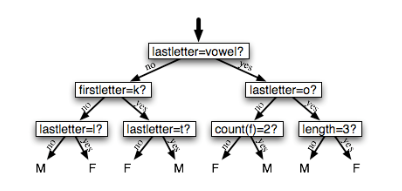
\includegraphics[width=0.5\linewidth]{images/Decisiontrees.png}
	\caption{Decision trees model to classify the gender of the names.}
	\label{fig:Decision_tree}
	\source{$http://www.nltk.org/book_1ed/ch06.html$}
\end{figure}

\subsection{Tools}
In order to realize this research, Python programming language and many other external tools and libraries are used. Python is an extremely powerful tool, also it is open source and flexible which adds to its popularity. It is known to have massive libraries for data manipulation and is extremely easy for all data analysts to learn and use. Some of the important libraries which is used in in this research are discussed in the following section.  


\begin{itemize}
    \item NLTK
    \item Scikit-learn: \\
    It  \cite{scikit-learn} is a free software machine learning library for python programming language. It is a tool for data pre-processing and data analysis, and offers many machine algorithms as well. The Scikit-learn project aims to provide state-of-the-art implementations for a wide range of machine learning methods, it has a clean API that is robust, fast, easy to use, comprehensive and well documented. The Document is provides more detailed information to the experienced data analyst, while at the same time simple, key points of a topic to the beginner. Some key elements of the framework are illustrated below.
    
    \begin{itemize}
        \item Countvectorizer
        \item Feature union
        \item train test split
    \end{itemize}
    
    
 
    
    \item Pandas \\
    \cite{pythonpandas}
\end{itemize}



\section{Related works in mining Twitter social media data}




\cite{Goergen} paper concentrates on event detection, which is mainly focused on 3 distinct parameters
known as w3 questions, "What is really happening, Where is the incident and When did the
event happen?". The authors collects the spatial-temporal data from Twitter from two different
countries. They use Names entity recognition, Geo-coordinates to identify location. Using this
data authors determine the "number of possible users for a shared account by calculating the
distance and velocity between tweets belonging to single account".

 
Authors from \cite{Hadgu} and  \cite{Böhm2017} presents an approach to classify the Twitter user to a particular domain, for example, Researcher or Economist. Authors of \cite{Hadgu} presents a method to classify a twitter user to a specific researcher discipline. They use a seed set from the computer science conference and crawl Twitter to collect relatively good ground truth data. This mapping is used to learn a model for classifying the Twitter user to particular desired discipline. Authors of \cite{Böhm2017}  extends this approach to classify Economist in Twitter. Their approach differs from \cite{Hadgu}, as they use the "Text" of the tweets for classification. They collect ground truth data by comparing the Twitter user account name with the economic publication database. This data is used to train a classifier model. But, In my case, It is very difficult to get the ground truth data, There is limited data where the Twitter user can be verified to figure out the Tweet is coming from a migrant or Tweet "Text" is related to migration. 
 
\cite{Hübl} paper concentrates on "Individual and aggregate trajectories that reflects the refugee migration
movements" and "identify the spatiotemporal event clusters of refugee-related tweets to
likely determine the location of refugees". The technique used by authors to collect data is, they
downloaded all the Twitter data in a specific time frame and apply filters to separate out tweets
which were of geographic interest. Authors collect both tweets which were geotagged with coordinates
and with geotagged with a place description. For the latter type, The twitter places were
are extended over continents. In addition to above filtering method, the authors also filter tweets
of interest based on hashtag search. \cite{Hübl} work inspired me on how to collect word list for filtering
tweets related to migration. But this work was related to the refugee crisis.
 
Compare to the data collection method used by \cite{Hübl}. The authors of \cite{Cortis} use hashtag filtering
along with popular terms used in those tweets. \cite{Cortis} tries to analyze cyberbullying tweets in trending
world events. The authors choose two world events which were the cause of several cyberbullying.
The technique used by authors to collect and filter Twitter data is that they select two real-world
events trending hashtags along with popular cyberbullying terms. This technique inspired me to
apply this filter logic to collect tweets regarding migration.
Regarding Sentiment analysis there are two approaches, One approach is to use the labeled
texts and use supervised machine learning trained on the labeled text data to classify the polarity
of new texts. Another approach creates a sentiment lexicon and scores the text based on some
function that describes how the words and phrases of the text match the lexicon, \cite{DBLP} Evaluates
word list sentiment analysis for microblogging.

 \cite{Jamie} Discusses how a classifier model is trained
and evaluated by calculating precision, recall and F1 score on manually annotated and classifier
predictions.


 \underline{matte heavy agi bari}
